\chapter{Grafik-Dateien}
\renewcommand{\chaptertitle}{Grafik-Dateien}

\lehead[]{\normalfont\sffamily\hspace*{-2.00cm}\textcolor{white}{\colorbox{lightblue}{\makebox[1.60cm][r]{\thechapter}}}\hspace{0.17cm}\textcolor{lightblue}{\chaptertitle}}
\rohead[]{\textcolor{lightblue}{\chaptertitle}\normalfont\sffamily\hspace*{0.17cm}\textcolor{white}{\colorbox{lightblue}{\makebox[1.60cm][l]{\thechapter}}}\hspace{-2.00cm}}
%\chead[]{}
\rehead[]{\textcolor{lightblue}{AvHG, Inf, My}}
\lohead[]{\textcolor{lightblue}{AvHG, Inf, My}}

\lstset{style=myJava}

\section{Grafik-Dateien in eigenen Java-Programmen nutzen}

\subsection{Unterstützte Bildformate}

Java unterstützt die Bildformate \myFile{GIF}, \myFile{JPEG} und \myFile{PNG}.
Bei \myFile{GIF}-Bildern kann man mit einem Bildbearbeitungsprogramm wie z.B.
Gimp oder Photoshop einen transparenten Hintergrund setzen, der beim Zeichnen
nicht mit gemalt wird.

\subsection{Erzeugung eines Image-Objektes}

Für Bildern gibt es die Klasse \myClass{Image}.

Um ein Objekt der Klasse \myClass{Image} zu erzeugen, benötigt man zunächst das
\lstinline|Toolkit| der aktuellen Umgebung. Die Klasse \myClass{JFrame} (das
Anwendungsfenster) besitzt eine Methode, um das \lstinline|Toolkit| zu
beschaffen:

\begin{lstlisting}
public Toolkit getToolkit()
\end{lstlisting}

Das \lstinline|Toolkit| wiederum besitzt eine Methode zum Erstellen eines
\myClass{Image}-Objektes:

\begin{lstlisting}
public Image getImage(String datei)
\end{lstlisting}

Ein \myClass{Image}-Objekt für die Datei \myFile{bild.gif} kann man im
Anwendungsfenster z.B.\ folgendermaßen erzeugen:

\begin{lstlisting}
Image bild1;
Toolkit kit = getToolkit();
bild1 = kit.getImage("bild.gif");
\end{lstlisting}

Verkürzt kann man auch schreiben:

\begin{lstlisting}
Image bild2;
bild2 = getToolkit().getImage("name.gif");
\end{lstlisting}

Zu bevorzugen ist jedoch eine zweite Variante von \lstinline|getImage()| – dabei
wird statt einen Strings eine URL übergeben:

\begin{lstlisting}
public Image getImage(URL url)
\end{lstlisting}

Die benötigte URL bekommt man auf den ersten Blick umständlich – dafür in der
Praxis sehr verlässlich – über den folgenden Aufruf:

\begin{lstlisting}
bild2 = getToolkit().getImage(getClass().getResource("name.gif"));
\end{lstlisting}

Zur Erklärung: \lstinline|getClass()| liefert die Klasse des aufrufenden
Objektes zurück. Über \lstinline|getResource()| wird die Datei, die als
String angegeben wurde, als \myClass{URL}-Objekt zurück gegeben. Das
funktioniert selbst dann, wenn diese Dateien aus einer \myFile{.jar} Datei
geladen werden. Wenn die Bild-Datei in einem Unterverzeichnis relativ zu der
aufrufenden Java-Klasse liegt, dann kann dies mit angegeben werden.
Beispielsweise:

\begin{lstlisting}
bild2 = getToolkit().getImage(getClass().getResource("images/name.gif"));
\end{lstlisting}

Da das Laden einer Bitmap sehr lange dauern kann, sollte die Bitmap nur einmal
im Konstruktor geladen werden. Um sicher zu stellen, dass die Bilder
vollständig geladen sind ehe die Anwendung zum ersten Mal gezeichnet wird,
sollte man anschließend im Konstruktor noch ein Objekt der Klasse
\myClass{MediaTracker} benutzen:

\begin{lstlisting}
MediaTracker mt = new MediaTracker(this);     æ// this ist das Anwendungsfenster
æmt.addImage(bild1);
mt.addImage(bild2);
try {
  mt.waitForAll();
} catch (Exception e) {
  e.printStackTrace();
}
\end{lstlisting}

Um zu überprüfen, ob es beim Laden eines der Bilder zu einem Fehler kam, sollte
man anschließend noch genau dies mit der Methode \lstinline|isErrorAny()| tun:

\begin{lstlisting}
if (mt.isErrorAny()) {
  System.out.println("Problem beim Laden eines Bildes!");
}
\end{lstlisting}


\subsection{Malen eines Image-Objektes}

Objekte der Klasse \myClass{Image} können mit der Methode
\lstinline|drawImage()| der Klasse \myClass{Graphics} angezeigt werden:

\begin{lstlisting}
public boolean drawImage(Image img, int x, int y, ImageObserver observer)
\end{lstlisting}

Neben dem \myClass{Image}-Objekt wird die Position der linken oberen Ecke (x, y)
angegeben. Als letzter Parameter wird ein Objekt des Fensters angegeben, das
den Ladezustand der Bitmap überwacht. Bei uns ist dies immer das Objekt des
Anwendungsfensters.


\subsection{Beispiel-Programm}

Datei \myFile{HausAnwendung.java}:

\begin{lstlisting}
æimport java.awt.*;
import hilfe.*;

public class æHausAnwendungæ extends HJFrame {
  private static final int WIDTH = 500;
  private static final int HEIGHT = 500;
  private static final Color BACKGROUND = new Color(199, 231, 203); // blassgrün
  private static final Color FOREGROUND = Color.BLACK;
  private Haus h1, h2, h3, h4;

  public HausAnwendung(final String title) {
    super(WIDTH, HEIGHT, BACKGROUND, FOREGROUND, title);
    h1 = new Haus(100, 50, this);
    h2 = new Haus(300, 300, this);
    h3 = new Haus(50, 250, this);
    h4 = new Haus(200, 100, this);
  }
  
  public void myPaint(Graphics g) {
    h1.zeichnen(g);
    h2.zeichnen(g);
    h3.zeichnen(g);
    h4.zeichnen(g);
  }

  public static void main(final String[] args) {
    EventQueue.invokeLater(new Runnable() {
      public void run() {
        try {
          HausAnwendung anwendung = new HausAnwendung("HausAnwendung");
        } catch (Exception e) {
          e.printStackTrace();
        }
      }
    });
  }
}
\end{lstlisting}

\vspace{5mm}

Datei \myFile{Haus.java}:

\begin{lstlisting}
æimport java.awt.Graphics;
import java.awt.Image;
import java.awt.MediaTracker;

public class æHausæ {
  private æHausAnwendung anwendungæ;
  private int x, y;
  private æImage hausBildæ;

  public Haus (int x, int y, æHausAnwendung anwendungæ) {
    this.x = x;
    this.y = y;
    this.anwendung = anwendung;
æ    hausBild = anwendung.getToolkit().getImage(getClass().getResource("haus.gif"));
    MediaTracker mt = new MediaTracker(anwendung);
    mt.addImage(hausBild);
    try {
      mt.waitForAll();
    } catch (Exception e) {
    }
    if (mt.isErrorAny()) {
      System.out.println("Problem beim Laden eines Bildes!");
    }æ
  }

  public void zeichnen (Graphics g) {
    æg.drawImage(hausBild, x, y, anwendung);æ
  }
}
\end{lstlisting}

\vspace{12mm}

\begin{center}
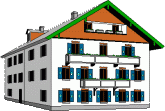
\includegraphics[width=0.4\textwidth]{./inf/SEKII/13_Java_Bilder/haus.png}
\end{center}

Anmerkung:

Die Methode \lstinline|getToolkit()| kann in diesem Beispiel nicht direkt
aufgerufen werden, weil sie nur auf Fenster (genauer: Komponenten) anzuwenden
ist. Die Klasse, die bei uns das Fenster liefert ist die Klasse
\myClass{HausAnwendung}. Deshalb wird in diese Beispiel das Objekt der
Anwendungsklasse gebraucht, um die Methode \lstinline|getToolkit()| benutzen zu
können. Wir brauchen ja das Toolit der Anwendungsklasse!
